\documentclass[11pt,a4paper]{article}

% ---------- Packages ----------
\usepackage[margin=1.9cm]{geometry}
\usepackage[T1]{fontenc}
\usepackage{charter}
\usepackage{microtype}
\usepackage{booktabs}
\usepackage{tabularx}
\usepackage{array}
\usepackage{enumitem}
\usepackage{xcolor}
\usepackage{titlesec}
\usepackage{tikz}
\usetikzlibrary{arrows.meta,positioning,calc}
\usepackage[colorlinks=true,linkcolor=black,urlcolor=blue!50!black,citecolor=black]{hyperref}

% ---------- Layout ----------
\setlength{\parindent}{0pt}
\setlength{\emergencystretch}{1.5em}
\setlength{\parskip}{3pt}
\setlist{nosep,leftmargin=*,topsep=2pt}
\titleformat{\section}{\large\bfseries}{\thesection.}{0.5em}{}
\titlespacing*{\section}{0pt}{8pt}{3pt}
\titleformat{\subsection}{\normalsize\bfseries}{\thesubsection}{0.5em}{}
\titlespacing*{\subsection}{0pt}{5pt}{2pt}
\newcolumntype{L}{>{\raggedright\arraybackslash}X}
\renewcommand{\arraystretch}{1.08}
\newcommand{\code}[1]{\texttt{\small #1}}
\newcommand{\done}{\textcolor{green!45!black}{\textbf{done}}}
\newcommand{\partdone}{\textcolor{orange!80!black}{\textbf{partial}}}
\newcommand{\notdone}{\textcolor{blue!60!black}{\textbf{next}}}
\newcommand{\repo}{\url{https://github.com/varunmodi18/Gate-Before-You-Act}}

\begin{document}

% ---------- Title block ----------
\begin{center}
{\small Language Models and Agents (CL3.410) \;|\; Group Project \;|\; Mid-Submission Report}\\[5pt]
{\LARGE\bfseries Gate Before You Act}\\[3pt]
{\large Does Verifying Evidence Make an LLM Security Agent Act More Safely\\ Than Policy Rules Alone?}\\[6pt]
{\small Team \textbf{Simpletons} \;|\; 26 October 2026}\\[4pt]
\begin{tabular}{llll}
\textbf{Varun Modi} & \textbf{Aayush Pandey} & \textbf{Srushti Pekamwar} & \textbf{Dhruv Rajput}\\
2025202040 & 2025201058 & 2025201066 & 2025201094
\end{tabular}\\[6pt]
{\small \textbf{GitHub repository:} \repo\ \;(branch \code{main}, commit \code{b9ca9e4})}
\end{center}

\noindent\fbox{\parbox{\dimexpr\linewidth-2\fboxsep-2\fboxrule}{\small
\textbf{Status in one paragraph.} The software is complete through milestone M7. \emph{GateBench}, our research workbench, ingests the OTRF logs and builds a Sigma/ATT\&CK retrieval index. It implements the gate checks C1--C6 and all ten systems (G0--G3, A1--A8), the episode loop with recovery budgets, an MCP transport, the end-to-end investigator, scoring, cluster-bootstrap analysis and a web interface for authoring, annotating, running and reading results. The model is Qwen2.5-7B-Instruct (4-bit AWQ) served by vLLM on an 8\,GB laptop GPU. It runs at 1,229 input and 55 output tokens/s, and the proposer produces schema-valid JSON on 80/80 pilot calls. Every experiment runner has completed live runs end to end on hand-made demo cases. 855 unit/integration tests, 19 front-end tests and 47 browser tests pass. \textbf{What comes next:} authoring and double annotation of the SOC-Risk case set, the freeze and the research runs, for which every component is now in place. The hypothesis tests (H1, H1-C4, H2) are therefore part of the final submission; the numbers in \S\ref{sec:results} come from pipeline-validation runs on demo fixtures and are not findings. \S\ref{sec:timeline} gives the dated plan to the final submission on 15 November, with the fallback triggers from the proposal and what each would change in our claims.}}

% =====================================================
\section{Project Recap}
An LLM agent investigates one suspicious Windows host from its Sysmon and Security logs and proposes a response, such as isolating the host or disabling an account. A \emph{gate} checks every state-changing action before it reaches the (mock) tools. A strong gate can enforce written policy alone. We ask whether \emph{also} checking that the cited log evidence supports the specific action improves decisions, with policy, trusted context, model and tools held fixed, and which part of that check helps: deterministic target matching (C3) or the LLM verifier (C4).

\textbf{Hypotheses (unchanged from the final proposal).} \textbf{H1}: on evidence packages that should be rejected (variants E2--E5), the full gate G3 wrongly admits $\geq$15 points fewer actions than the policy-only gate G1. \textbf{H1-C4}: on E4--E5, G3 wrongly admits $\geq$10 points fewer than A1 (G3 without the LLM verifier). \textbf{H2}: in full episodes, G3's unnecessary-deferral rate is not more than 10 points worse than G1's. Experiment~3 (live end-to-end investigation) is descriptive. Every effect is reported with a 95\% cluster-bootstrap interval over source scenarios.

\begin{center}
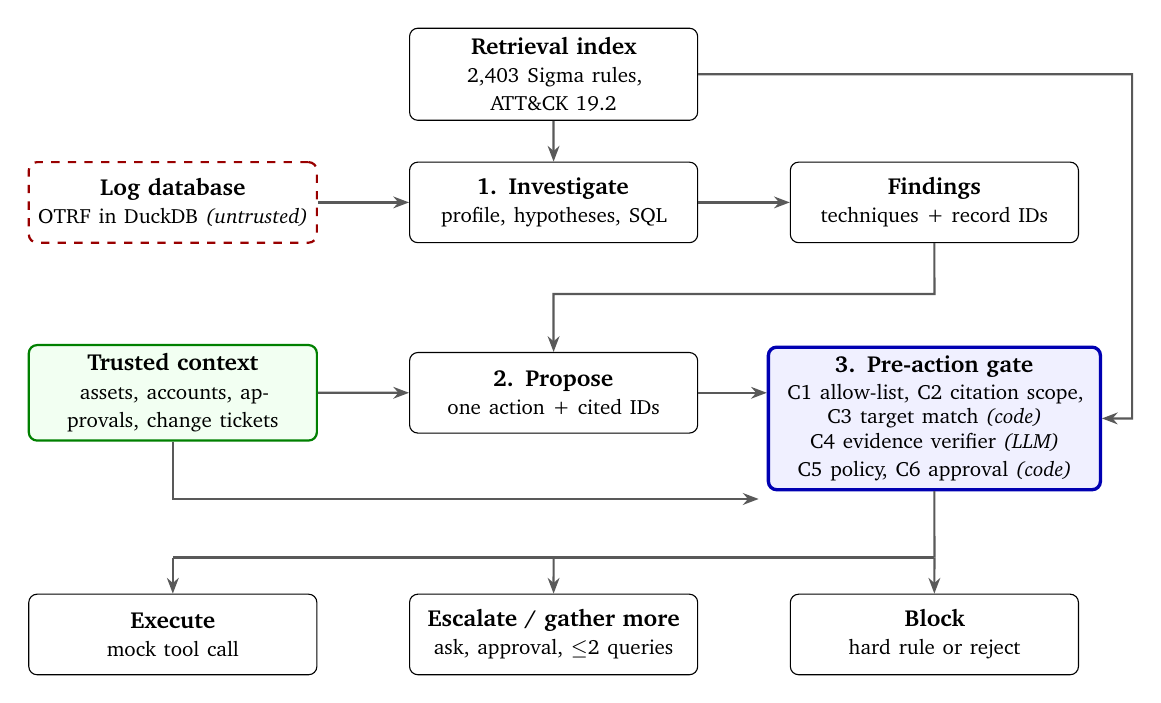
\begin{tikzpicture}[scale=0.93, transform shape,
  box/.style={draw, rounded corners=3pt, align=center, font=\small, minimum height=11mm, text width=3.7cm, fill=white},
  gate/.style={box, draw=blue!70!black, very thick, fill=blue!6, text width=4.3cm},
  trust/.style={box, draw=green!50!black, thick, fill=green!5},
  untr/.style={box, draw=red!60!black, thick, dashed},
  arr/.style={-{Stealth[length=2mm]}, thick, gray!70!black}]
\node[box] (sig) at (5.2,1.75) {\textbf{Retrieval index}\\ \footnotesize 2,403 Sigma rules, ATT\&CK 19.2};
\node[untr] (logs) at (0,0) {\textbf{Log database}\\ \footnotesize OTRF in DuckDB \emph{(untrusted)}};
\node[box] (inv) at (5.2,0) {\textbf{1. Investigate}\\ \footnotesize profile, hypotheses, SQL};
\node[box] (find) at (10.4,0) {\textbf{Findings}\\ \footnotesize techniques + record IDs};
\node[trust] (ctx) at (0,-2.6) {\textbf{Trusted context}\\ \footnotesize assets, accounts, approvals, change tickets};
\node[box] (prop) at (5.2,-2.6) {\textbf{2. Propose}\\ \footnotesize one action + cited IDs};
\node[gate] (gate) at (10.4,-2.95) {\textbf{3. Pre-action gate}\\[1pt] \footnotesize C1 allow-list, C2 citation scope,\\ \footnotesize C3 target match \emph{(code)}\\ \footnotesize C4 evidence verifier \emph{(LLM)}\\ \footnotesize C5 policy, C6 approval \emph{(code)}};
\node[box] (exe) at (0,-5.9) {\textbf{Execute}\\ \footnotesize mock tool call};
\node[box] (esc) at (5.2,-5.9) {\textbf{Escalate / gather more}\\ \footnotesize ask, approval, $\leq$2 queries};
\node[box] (blk) at (10.4,-5.9) {\textbf{Block}\\ \footnotesize hard rule or reject};
\draw[arr] (logs) -- (inv);
\draw[arr] (inv) -- (find);
\draw[arr] (sig) -- (inv);
\draw[arr] (sig.east) -- (13.1,1.75) |- (gate.east);
\draw[arr] (find.south) -- (10.4,-1.25) -| (prop.north);
\draw[arr] (ctx) -- (prop);
\draw[arr] (prop.east) -- (prop.east -| gate.west);
\draw[arr] (ctx.south) |- (8.0,-4.05);
\draw[thick, gray!70!black] (gate.south) -- (10.4,-4.85);
\draw[thick, gray!70!black] (0,-4.85) -- (10.4,-4.85);
\draw[arr] (0,-4.85) -- (exe.north);
\draw[arr] (5.2,-4.85) -- (esc.north);
\draw[arr] (10.4,-4.85) -- (blk.north);
\end{tikzpicture}
\end{center}
\vspace{-6pt}
{\small\textit{Figure 1.} Architecture as implemented. Red dashed = attacker-influenced data; green = trusted data. Only the gate can let a state-changing call reach the mock tools; over MCP (A8) the gate runs inside the tool server.}

% =====================================================
\section{Progress}
\label{sec:progress}
The work follows a dependency-ordered plan (\code{IMPLEMENTATION\_PLAN.md}, Draft~9). Each milestone was built on its own branch, and each branch contains the one before it; all of them are now merged into \code{main}. \code{STATUS.md} records every task, decision and measured number with its date.

{\small
\begin{tabularx}{\linewidth}{@{}p{3.3cm}p{1.6cm}L@{}}
\toprule
\textbf{Milestone (branch)} & \textbf{Status} & \textbf{Observable result}\\
\midrule
M0 Foundations (\code{m0-foundations}) & \done & Repo scaffold, store and migrations, LLM client (live / fake / replay), model-serving spike and pilot \\
M1 Data (\code{m1-data}) & \done & Pinned OTRF fetch, catalogue, normaliser to DuckDB, SQL guard, de-duplication, frozen window splits, Windows page \\
M2 Deterministic gate (\code{m2-gate}) & \done & Trusted-context model, policy engine (signed off), tool layer and provenance registry, C1--C3, C5, C6, Gate Playground \\
M3 Verifier and Exp 1 (\code{m3-verifier}) & \done & Retrieval index, C4 verifier with its four input variants, CPU reranker, retrieval metrics, Exp 1 runner; live demo-set Exp 1 \\
M4 Cases and annotation (\code{m4-cases}) & \done\ (code) & Scenario Studio, variant builder E1--E5 and Set R, database patcher, validator, blind double annotation, $\kappa$/Jaccard snapshots, adjudication, freeze tool \\
M5 Episodes and Exp 2 (\code{m5-episodes}) & \done & Proposer, episode loop, outcome classifier, Exp 2 runner with fallback F1, recovery budgets (A5/A7), MCP server (A8), Agent Console; live demo-set Exp 2 \\
M6 Investigation and Exp 3 (\code{m6-investigation}) & \done & Live investigator (three tuning rounds, then frozen), Exp 3 runner, technique and evidence metrics, Console window mode \\
M7 Analysis (\code{m7-analysis}) & \done\ (code) & All proposal metrics, cluster bootstrap, H1/H1-C4/H2 verdict logic, Results page, error taxonomy, exports. Sensitivity re-estimate waits for dev scenarios \\
M8 Hardening and docs & \partdone & Playwright suite with accessibility checks, performance check, README, runbook, generated gate contract and API docs. Open: live demo recording, a teammate's setup dry run \\
Case set: authoring, annotation, freeze & \notdone & 10 dev, 40 test and 12 end-to-end scenarios on the frozen window splits; all tooling for authoring, blind double annotation and adjudication is built and tested \\
Research runs Exp 1--3 & \notdone & Runners verified live on demo fixtures; start once the case set is frozen \\
\bottomrule
\end{tabularx}}

\textbf{Engineering quality.} About 20,400 lines of Python (\code{backend/gbya/}) and 6,900 lines of TypeScript/React (\code{frontend/}). Latest run (26 Oct): \code{make lint} clean (ruff, mypy strict on the gate, scoring, analysis and case modules, eslint, tsc); \textbf{855 pytest tests pass} (3 GPU-only tests deselected) and \textbf{19 vitest tests pass}. On 14 Oct, \textbf{46 Playwright journeys} passed at two viewports with axe accessibility checks on every page, plus 1 replay-profile demo run. Mutation checks were run on the security-critical parts (provenance registry, typed-argument rule), and the corresponding tests fail when the logic is deliberately broken. Measured latency (NFR-10): code-only gate check p95 3.2\,ms, guarded SQL on the largest window (79,896 events) p95 9.0\,ms, API list endpoints p95 11.5\,ms, first UI load 151\,ms.

\textbf{What the implementation guarantees.} A SELECT-only, two-layer SQL guard (AST checks plus a hardened read-only DuckDB connection; 70 attack tests). Typed-argument provenance: a PID, host, account or IP can fill an action argument only if it appeared in a record the agent actually retrieved. A rationale-blind verifier whose prompt never truncates cited fields. An approval state machine in which ``reachable'' never counts as ``granted''. No delete tool exists; attempts are counted.

% =====================================================
\section{Datasets in Use}
\label{sec:data}
{\small
\begin{tabularx}{\linewidth}{@{}p{3.2cm}L@{}}
\toprule
\textbf{Source} & \textbf{As loaded (measured)}\\
\midrule
OTRF Security-Datasets \cite{otrf} (MIT) & Pinned at commit \code{d9d40ef}. 100 Windows atomic datasets catalogued; \textbf{99 ingested} into per-window DuckDB files (7 normalised tables plus \code{raw\_events}): \textbf{757,375 events}, 0 skipped lines, 2.3\,GB, built in 35\,s. One window (SDWIN-230718150800) has its host file missing at the pinned commit and is excluded rather than mapped to a look-alike file. Four collection formats are handled. \\
De-duplication and splits & Event-signature Jaccard $>$0.5 groups 5 pairs: 99 windows form 94 groups. Seeded, tactic-stratified split, accepted by the team on 8 Oct: \textbf{dev 10, test 40, end-to-end 12}, 37 unused (one fallback queue). All 8 tactics with eligible windows appear in dev and test. \\
SigmaHQ rules \cite{sigma} (DRL 1.1) & Release \code{r2026-07-01}, \code{rules/windows/} only: \textbf{2,403 rules}. ATT\&CK tags and technique IDs are removed from the indexed text, so retrieval is by content. \\
MITRE ATT\&CK \cite{attack} & Enterprise STIX 2.1, version 19.2; 474 Windows techniques indexed. \\
SOC-Risk (ours) & Tooling complete: scenario files, variant builder (E1--E5 by database patching), Set R twins, validator (checks a--k, scope rule), annotation and adjudication. Authoring and annotation are the next step (\S\ref{sec:timeline}). Design target: 40 test scenarios $\times$ 7 cases = 280 cases, plus 12 end-to-end windows. \\
Demo fixtures (development only) & 3 hand-made cases; the \code{demo-lsass} scenario (LSASS memory dump on WORKSTATION5, 7 cases, labels set for demonstration only); 5 \emph{unused} windows used only to tune the investigator. None is a research window. \\
\bottomrule
\end{tabularx}}

% =====================================================
\section{Baselines and Ablations}
\label{sec:systems}
All systems share the model, tools, trusted context, signed-off policy (9 rules; all 144 attribute combinations are decided by a rule), hard rule and token caps; only the gate configuration differs. Each configuration is a data entry in \code{gate/configs.yaml}, and snapshot tests confirm that each ablation differs from G3 in exactly one field.

{\small
\begin{tabularx}{\linewidth}{@{}p{0.7cm}Lp{1.5cm}p{3.6cm}@{}}
\toprule
\textbf{ID} & \textbf{System} & \textbf{Built} & \textbf{Exercised live so far}\\
\midrule
G0 & ReAct agent, no gate & yes & Exp 1 (reference), Exp 2 demo \\
G1 & Policy-only gate: C1, C5, C6 & yes & Exp 1, Exp 2 demo \\
G2 & G1 + C2 citation scope & yes & Exp 1, Exp 2 demo \\
G3 & Full gate C1--C6 (simple RAG, recovery budget 2) & yes & Exp 1, 2, 3 demo \\
A1 & G3 without C4 (code checks only) & yes & Exp 1, Exp 2 demo \\
A2 & G3 without C3 & yes & Exp 1 demo \\
A3 & Verifier also sees the agent's rationale & yes & Exp 1 demo \\
A4 & No RAG (verifier gets no retrieved text) & yes & Exp 1 demo \\
A6 & RAG with reranker (BM25 top-20 $\to$ bge-reranker-base on CPU) & yes & Exp 1 demo \\
A5 / A7 & Recovery budget 0 / 1 (G3 = 2) & yes & Exp 2 demo (A5) \\
A8 & G3 with tools served over MCP, gate inside the server & yes & Exp 2 demo \\
\bottomrule
\end{tabularx}}

% =====================================================
\section{Experiments Run and Results So Far}
\label{sec:results}
\textbf{Reading this section.} Every run below is a \emph{pipeline-validation} run on development fixtures: 3 hand-made cases and the 7-case \code{demo-lsass} scenario, whose labels were set for demonstration and not double-annotated. The software itself refuses to compute hypothesis verdicts on such runs. These numbers show that each component works end to end with the live model, and they surface early behaviour worth watching. They do \emph{not} estimate any effect in H1, H1-C4 or H2.

\subsection{Model serving pilot (8 Oct)}
Qwen2.5-7B-Instruct, 4-bit AWQ, vLLM 0.31, 8k context, xgrammar JSON-constrained decoding, on the RTX 4060 Laptop GPU (8\,GB).

{\small
\begin{tabularx}{\linewidth}{@{}Lr@{}}
\toprule
\textbf{Measure (20 synthetic episodes + 7,850-token request + 30-min soak)} & \textbf{Value}\\
\midrule
Throughput, 4 concurrent requests (input / output tokens per s) & 1,229.2 / 55.4 \\
Proposal's planning assumption (input / output) & 800 / 80 \\
Latency p50 / p95 & 14.0 / 19.0\,s \\
Peak VRAM / peak host RAM & 7,249\,MiB / 8,201\,MB \\
Schema-valid outputs, generic schema (pilot / soak) & 78/80 / 459/480 \\
Schema-valid outputs, final proposer schema (T5.1 acceptance, 13 Oct) & \textbf{80/80} \\
Soak: minimum output rate, maximum GPU temperature & 53.0 tok/s, 80\,$^\circ$C \\
\bottomrule
\end{tabularx}}
Output throughput is 31\% below the proposal's assumption but above the fallback-F1 threshold (half the assumption), so F1 was not triggered on throughput grounds. A trial token audit on the demo data (14 Oct), with every output assumed to hit its length cap, projects 65.2\,GPU-hours for the full design, or 97.9\,h with the 1.5$\times$ allowance. That is a pessimistic bound, and the real audit (T8.0) needs the dev scenarios.

\subsection{Experiment 1 pipeline: gate decisions, verifier and retrieval}
Live run through the worker on the 3 hand-made cases with all nine Exp~1 configurations: \textbf{93/93 units completed, 0 errors, in 20\,s}. That is 36 verifier calls (standard, rationale, no-RAG and reranked inputs, 3 runs each), 12 code-only decisions and 45 composed decisions; every verifier output parsed. Repeated runs of the same (case, variant) gave identical verdicts at temperature 0. G3, A3, A4 and A6 reached C4 on 6 of 9 packages, because C3 stopped the wrong-target package first; A2 (no C3) reached C4 on 9 of 9. This confirms that the component split H1-C4 depends on is wired correctly.

{\small
\begin{tabularx}{\linewidth}{@{}Lrrrrr@{}}
\toprule
\textbf{Retrieval level (3 cases)} & \textbf{Recall@5} & \textbf{Hit@5} & \textbf{nDCG@5} & \textbf{MRR@20} & \textbf{ATT\&CK top-1}\\
\midrule
Simple RAG: BM25 (G3) & 0.023 & 0.333 & 0.333 & 0.333 & 0.333\\
RAG + reranker (A6) & 0.019 & 0.333 & 0.277 & 0.333 & 0.333\\
\bottomrule
\end{tabularx}}
These are illustrative, not comparative: $n=3$, and two of the three hand-made cases cite domain-controller logon records under an LSASS gold technique. The run did expose a real measurement issue (\S\ref{sec:challenges}): the gold set for T1003.001 contains 71 Sigma rules, so Recall@5 can be at most $5/71 \approx 0.07$. Reranking costs about 7.0\,s per case on the CPU (peak 2.0\,GB RAM) against 0.024\,s for BM25 alone. Rankings are cached, so Exp~1 spends no GPU time on retrieval.

\subsection{Experiment 2 pipeline: full episodes}
Live run on the 7 \code{demo-lsass} cases (E1--E5, R\textsubscript{pos}, R\textsubscript{neg}). G0, G1 and G3 ran $\times$3 and G2, A1 and A5 ran $\times$1: \textbf{84/84 episodes completed, 0 errors, every unit on its first attempt, in 2\,min 26\,s}. There were 163 proposer calls (1--4 per episode) with \textbf{0 unusable outputs} and no history truncation, plus 77 gate decisions with 0 verifier parse errors. Terminal states: 68 actions fulfilled, 13 hand-offs to the analyst, 3 explicit ends. The gate failures were all of the expected kinds: 5 \code{C3\_HOST\_MISMATCH}, 2 \code{C6\_APPROVAL\_REQUIRED} and 2 \code{C6\_APPROVAL\_PENDING}.

\textbf{Early behaviour observed.} (i)~In 69 of 84 episodes the agent's first proposal was an unnecessary \code{request\_approval} for a tier-2 host. A prompt fix (shared identically by all systems) was made before the proposer prompt was frozen. (ii)~In the MCP comparison (A8 vs G3, one run each, 7 cases), both transports gave \textbf{identical outcomes on all 7 cases} (task success 4/7 for both, 13 tool calls and 8 admitted for each), at a median MCP round trip of 2.76\,s per gated call. In both, however, the live verifier returned \textsc{supports} on the demo E4 (partial chain) and E5 (in-scope approved activity) cases, which the demo labels count as unsafe executions. This is exactly the failure mode H1-C4 is designed to measure, and it is a warning that the 7B verifier may be weak on interpretation-heavy variants. One scenario cannot tell us how often it happens.

\subsection{Experiment 3 pipeline: live investigation}
The investigator builds a window profile, proposes 3--5 ATT\&CK hypotheses using retrieved candidate techniques (never the window's metadata), runs at most two guarded queries per hypothesis and verifies each technique against cited records within a 25-call budget. It was tuned on 5 unused windows (one per tactic) over three logged rounds and then frozen (prompt hashes in \code{STATUS.md}):

{\small
\begin{tabularx}{\linewidth}{@{}p{2.2cm}L@{}}
\toprule
\textbf{Round} & \textbf{Change $\to$ result on the 5 tuning windows (G3, 1 run each)}\\
\midrule
Smoke + 1 & Profile and SQL-prompt fixes $\to$ expected technique found on 0/5; the response agent sometimes looped until the 8-call cap \\
2 & Window summary passed to the SQL step, escalation guidance $\to$ 0/5; loop fixed \\
3 (frozen) & $\geq$3 hypotheses enforced by schema; top-10 retrieved ATT\&CK candidates offered $\to$ \textbf{1/5} (LSASS dump found and accepted on the right records); pooled precision 0.33, recall 0.20, F1 0.25 \\
\bottomrule
\end{tabularx}}
Diagnosis: in 10 of 11 pre-round-3 investigations the expected technique was never even hypothesised, so hypothesis generation, not verification, is the bottleneck for this model. Episodes take 17--27\,s each. As planned, Exp~3 will be reported descriptively as it comes out.

% =====================================================
\section{Challenges Faced and Mitigations}
\label{sec:challenges}
{\small
\begin{tabularx}{\linewidth}{@{}LL@{}}
\toprule
\textbf{Challenge} & \textbf{What we did / will do}\\
\midrule
FP8 KV cache (planned, to fit 8\,GB) garbled the output at every prompt length tested (452--4,418 tokens) & FP16 KV cache with the same model file, accepted as a deviation. The KV cache then holds 21,520 tokens ($\approx$2.6 full-length requests at once), so long requests queue \\
Constrained decoding emitted only whitespace; 7B repetition loops hit \code{max\_tokens} (78/80 valid) & xgrammar backend with whitespace disabled; bounded strings and bounded integer IDs in the proposer schema $\to$ 80/80. Remaining invalid outputs count as rejections and are reported \\
Toolchain: FlashInfer JIT failed on the repository path containing spaces; \code{nvcc} not on \code{PATH} & vLLM environment moved to a space-free path; CUDA 13.0 set explicitly; every step recorded in the pilot report \\
Log data quirks: nxlog \code{ProcessID} is the log writer's PID, not the subject's; one dataset file is missing at the pinned commit & PID read from the event's own message (wrong PIDs would corrupt C3); the window is excluded and documented, never guessed \\
\textbf{The gate only sees cited records}: an agent can omit a contradicting record it retrieved & No gate change (it would alter the design mid-study); a \emph{retrieved-but-not-cited} measure is now reported per variant and system \\
Recall@5 is capped by large gold sets (71 rules for T1003.001; ceiling $\approx$0.07) & Report the ceiling next to Recall@5 and lead with Hit@5, nDCG@5 and MRR@20, as planned \\
Weak technique identification by the 7B investigator (F1 0.25 on 5 tuning windows) & Three logged tuning rounds, then frozen to avoid tuning on test data; Exp~3 stays descriptive \\
The agent can read the approval script via \code{get\_context}, so it knows the approver's answer in advance & Kept to match the proposal; listed as a limitation for the final report \\
Research labels must stay independent of the systems being tested & The server enforces blind double annotation, snapshots agreement before adjudication, and refuses research runs on unfrozen, replayed or fake-model data \\
\bottomrule
\end{tabularx}}

% =====================================================
\section{Plan and Timeline to the Final Submission (15 November)}
\label{sec:timeline}
Twenty days remain, which is enough to run the \textbf{full design from the final proposal}: 40 test scenarios (280 cases), 12 end-to-end windows, all systems and ablations. The proposal's two fallbacks stay in force, each with a dated trigger. The plan's dependency order is unchanged: annotation $\to$ freeze $\to$ research runs $\to$ analysis.

{\small
\begin{tabularx}{\linewidth}{@{}>{\raggedright\arraybackslash}p{2.7cm}L>{\raggedright\arraybackslash}p{3.5cm}@{}}
\toprule
\textbf{When} & \textbf{Work} & \textbf{Check}\\
\midrule
Mon 26 -- Tue 27 Oct & Shared annotation server up; all four calibrate together on dev-01 and dev-02 (author, blind second label, adjudication) & Both adjudicated; rule questions logged in \code{STATUS.md} \\
Wed 28 -- Fri 30 Oct & Dev-03 \dots\ dev-10 authored, double-annotated and adjudicated; pilot on the dev scenarios (purpose \emph{development}); T7.3 sensitivity re-estimate; T8.0 token audit and GPU budget. \emph{Mid-submission on 30 Oct} & Pilot runs end to end; measured interval half-widths and GPU-hours recorded \\
Sat 31 Oct -- Fri 6 Nov & All 40 test scenarios and 12 end-to-end windows authored, labelled by two annotators blind, then adjudicated ($\approx$90 person-hours in total, $\approx$22 per member); variants checked by both annotators & $\kappa\geq0.6$ on the agreement snapshots before adjudication \\
Wed 4 Nov & \textbf{F2 checkpoint:} if fewer than 20 of the 40 test scenarios are adjudicated, switch to 30 test scenarios & Decision dated in \code{STATUS.md} \\
Sat 7 Nov & \textbf{Freeze} (\code{cases-v1}); retrieval cache on the frozen set; \textbf{Exp~1} (nine configurations; verifier $\times$3) & Freeze manifest committed; Exp~1 errors $<$1\% \\
Sat 7 -- Wed 11 Nov & \textbf{Exp~2}, all 14 system-runs (G0, G1, G3 $\times$3; G2, A1, A5, A7, A8 $\times$1), laptop dedicated to runs day and night; adjudication queue cleared daily. \textbf{F1 checkpoint:} if the T8.0 budget exceeds the hours left, drop to the F1 schedule & Every unit completed; queue empty \\
Thu 12 Nov & \textbf{Exp~3}: G0, G1, G3 $\times$2 on the 12 end-to-end windows & Completed; incidental-technique queue empty \\
Fri 13 -- Sun 15 Nov & Bootstrap analysis of H1, H1-C4 and H2; retrieval and agentic ablation tables; error taxonomy with 10 annotated traces; live demo recording; final report; tag and submit & Results page in research mode; report submitted \\
\bottomrule
\end{tabularx}}

\textbf{GPU time.} The proposal budgeted about 81\,GPU-hours including a 1.5$\times$ allowance. A pessimistic trial audit on the demo data (every output at its length cap) gives 97.9\,h. The real figure comes from T8.0 on the dev scenarios by 30 Oct. Running the laptop day and night from 7 to 12 Nov gives over 100\,h, but overnight-only running would give about 48\,h. So the T8.0 number decides, before the freeze, whether F1 applies.

\textbf{What the fallbacks change in the claims.} \textbf{F2} (30 test scenarios) widens the intervals by about $\sqrt{40/30}\approx1.15$. On the proposal's preliminary assumptions that is roughly 13 points for H1, 15 for H1-C4 and 9 for H2, which makes an ``inconclusive'' verdict on H1-C4 more likely. \textbf{F1} drops the single-run ablations from Exp~2 and uses 2 runs of G0, G1 and G3, which widens the H2 interval; Exp~1 (H1, H1-C4) is unaffected. Whichever applies is stated in the final report. If H1 is not supported, the deliverables in the proposal's fallback clause still stand: a controlled measurement of policy-only gating, the target-matching vs.\ verifier split, and a released case set with exact action labels.

% =====================================================
\section{Repository and Reproduction}
\textbf{Repository:} \repo\ (branch \code{main}). Each milestone also remains on its own branch (\code{m0-foundations} \dots\ \code{m7-analysis}).

{\small
\begin{tabularx}{\linewidth}{@{}>{\raggedright\arraybackslash}p{4.2cm}L@{}}
\toprule
\textbf{Path} & \textbf{Contents}\\
\midrule
\code{backend/gbya/} & data, retrieval, context, policy, tools (incl.\ MCP server), gate, llm, agent, cases, scoring, analysis, experiments, API, worker \\
\code{frontend/} & Vite + React + TypeScript interface: Windows, Scenario Studio, Annotate, Gate Playground, Agent Console, Experiments, Traces, Results \\
\code{policy/}, \code{experiments/}, \code{config/} & Signed-off policy rules and evidence requirements; experiment specifications incl.\ fallbacks; model profiles \\
\code{tests/} & Unit, integration and Playwright end-to-end suites \\
\code{docs/} & Final proposal, pilot report, gate contract, policy table, field map, splits, case-authoring guide, runbook, team guide, API reference \\
\code{IMPLEMENTATION\_PLAN.md}, \code{STATUS.md} & The plan, and the dated record of every task, decision and measured number \\
\bottomrule
\end{tabularx}}

\textbf{Running it.} \code{make setup \&\& make fixture-up} opens the interface on fixture data with a scripted model (no GPU, no downloads). \code{make db data index \&\& make demo-setup \&\& make model-up \&\& make demo-up} runs the live demo on the real LSASS window. \code{make test}, \code{make lint} and \code{make e2e} run the test suites. Logs, model weights and the index are rebuilt locally from pinned sources and never committed.

% ---------- References ----------
\begingroup
\footnotesize
\renewcommand{\section}[2]{\vspace{4pt}\textbf{\large References}\par\vspace{2pt}}
\begin{thebibliography}{99}
\setlength{\itemsep}{0pt}
\bibitem{otrf} OTRF Security-Datasets, commit d9d40ef. \url{https://github.com/OTRF/Security-Datasets}
\bibitem{sigma} SigmaHQ, Sigma rules, release r2026-07-01 (Detection Rule License 1.1). \url{https://github.com/SigmaHQ/sigma}
\bibitem{attack} MITRE ATT\&CK\textregistered{} Enterprise, STIX 2.1, v19.2. \copyright{} 2026 The MITRE Corporation; reproduced with permission. \url{https://github.com/mitre-attack/attack-stix-data}
\bibitem{opensec} J.~Barnes. OpenSec: Measuring Incident Response Agent Calibration Under Adversarial Evidence. arXiv:2601.21083, 2026.
\bibitem{aura} R.~Shang et al. AURA-Eval: Evaluation Framework for Acting Under Risk Awareness in LLM Agent Trajectories. arXiv:2609.06783, 2026.
\bibitem{camel} E.~Debenedetti et al. Defeating Prompt Injections by Design. arXiv:2503.18813, 2025.
\bibitem{react} S.~Yao et al. ReAct: Synergizing Reasoning and Acting in Language Models. arXiv:2210.03629, 2022.
\bibitem{reranker} BAAI bge-reranker-base. \url{https://huggingface.co/BAAI/bge-reranker-base}
\bibitem{mcp} Model Context Protocol specification. \url{https://modelcontextprotocol.io}
\bibitem{vllm} vLLM. \url{https://github.com/vllm-project/vllm}
\end{thebibliography}
\endgroup

\end{document}
